\documentclass[14pt,a4paper]{article}

\usepackage[utf8]{inputenc}
\usepackage[
backend=biber,
style=ieee,
natbib=true,
sorting=none,
url=false,
isbn=false,
doi=true
]{biblatex}
\addbibresource{bibliography.bib}
\usepackage[english,russian]{babel}
\usepackage[T2A]{fontenc}
\usepackage{graphicx}
\usepackage{amssymb}
\usepackage{amsthm}
\usepackage{amsmath}
\usepackage{bm}
\usepackage{tabularx}
\usepackage{adjustbox}
\graphicspath{{media}}
\usepackage{float}
\usepackage{caption} % пакет для работы с названиями плавающих элементов
\usepackage{}
%\setlength{\parindent}{1.25cm}
\usepackage{indentfirst}
\usepackage{wrapfig}
\usepackage[a4paper,
%showframe, % отображение границ области листа
top		=	2.00cm,
bottom	=	2.00cm,
left	=	3.00cm,
right	=	1.50cm,
nohead,
foot	=	0.75cm
]{geometry} % пакет формата листа

\setlength{\parindent}{1.25cm} % задаём размер красной строки
\usepackage{setspace} % пакет для работы с интервалами
\onehalfspacing % полуторный интервал

\usepackage{graphicx}

\begin{document}
    
    Отчет за третий квартал по проекту НЦМУ\\
    
    Выполнил Бондаренко Никита Александрович
    
    \section*{Аннотация}
    
    В данной работе рассматривается параметрическая геометрия микроканала с неоднородностью. Численно исследован нестационарный двухфазный режим течения в двумерной постановке. Получена зависимость остаточной нефтенасыщенности от отношения площадей пор при разных контактных углах.
    
    \section*{Параметрическая геометрия.}
    
    Микроканал с неоднородностью представляет собой	прямой канал с препятствием в виде цилиндра и с локальным расширением внешних стенок в месте нахождения препятствия (рис.~\ref{fig:HSgeom}). 
    
    \begin{figure}[H]
        \centering
        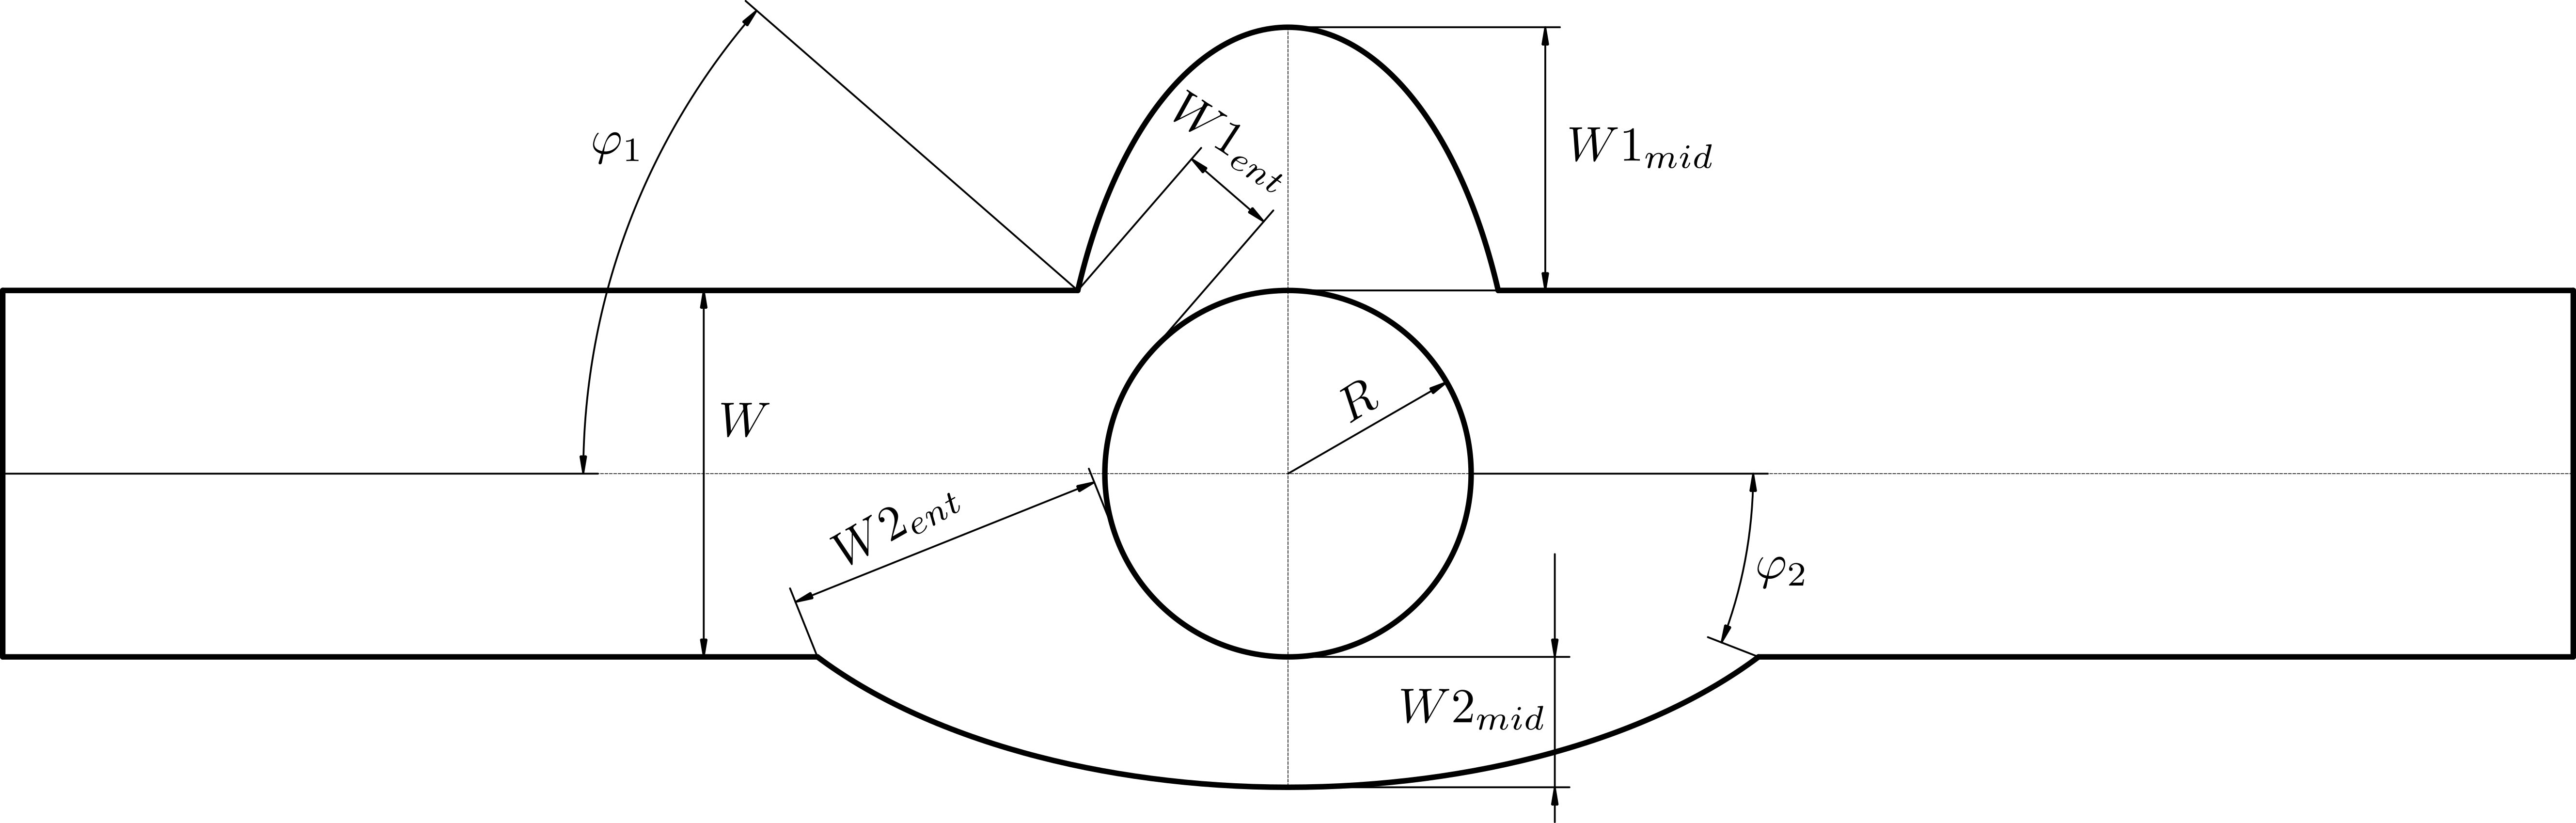
\includegraphics[width = 1\linewidth]{heleShawCellGeom}
        \caption{Микроканал с неоднородностью.}
        \label{fig:HSgeom}
    \end{figure}
    
    В разработанной параметрической модели построение геометрии осуществляется на основе следующих параметров. $W$ - это ширина основного канала,$W_{ent}$ - это ширина входа в пору (отрезок $W_{ent}$ перпендикулярен касательной препятствия), $W_{mid}$ - это ширина поры в центре. $\varphi$ - это угол между осью микроканала, которая проходит через центр препятствия, и отрезка $W_{ent}$, этот угол не является вводимым параметром.
    
    Расширение микроканала осуществлено при помощи эллипсов. Для их построения аналитически были выведены формулы для осей эллипса, $a$ и $b$.
    
    \begin{equation}\label{eqn:a}
        a^2 = \frac{(W_{ent} + R)^2 - \frac{W^2}{4}}{1 - \frac{W^2}{4  b^2}}
    \end{equation}  
    
    \begin{equation}
        b = R + W_{mid}
    \end{equation}
    
    Для дальнейшего исследования была выведена формула для расчета площади пор. Начало и конец поры определено отрезком $W_{ent}$ (рис.~\ref{fig:HSarea}).
    
    \begin{figure}[H]
        \centering
        
\includegraphics[width = 1\linewidth]{GeomArea}
        \caption{Площадь поры.}
        \label{fig:HSarea}
    \end{figure}
    
    \begin{equation}
    \begin{split}    
            S = \frac{1}{2} \pi ab - \frac{1}{2} \pi R^2 - \frac{C W_{ent}}{2} + \frac{b}{a}\left( a^2\pi - C\sqrt{a^2 - C^2} - a^2\arcsin(\frac{C}{a}) \right) - \arccos(\varphi)R^2,  C^2 = (R + W_{ent})^2 - (\frac{w}{2})^2 
    \end{split}
    \end{equation}
    
    \section*{Начальные условия.}
    
    В начальный момент времени поры микроканал полностью заполнен нефтью. С правой стороны задается объемный расход воды (2e-12 м$^3/c$), вытесняющей нефть. Контактный угол,$\alpha$, задается для воды. 
    
    \begin{figure}[H]
        \centering
        
\includegraphics[width = 1\linewidth]{zeroTimeCondition}
        \caption{Начальный момент времени, S1/S2 = 1, $\alpha$ = 140\textdegree}
        \label{fig:zeroTime}
    \end{figure}
     
     \begin{figure}[H]
         \centering
         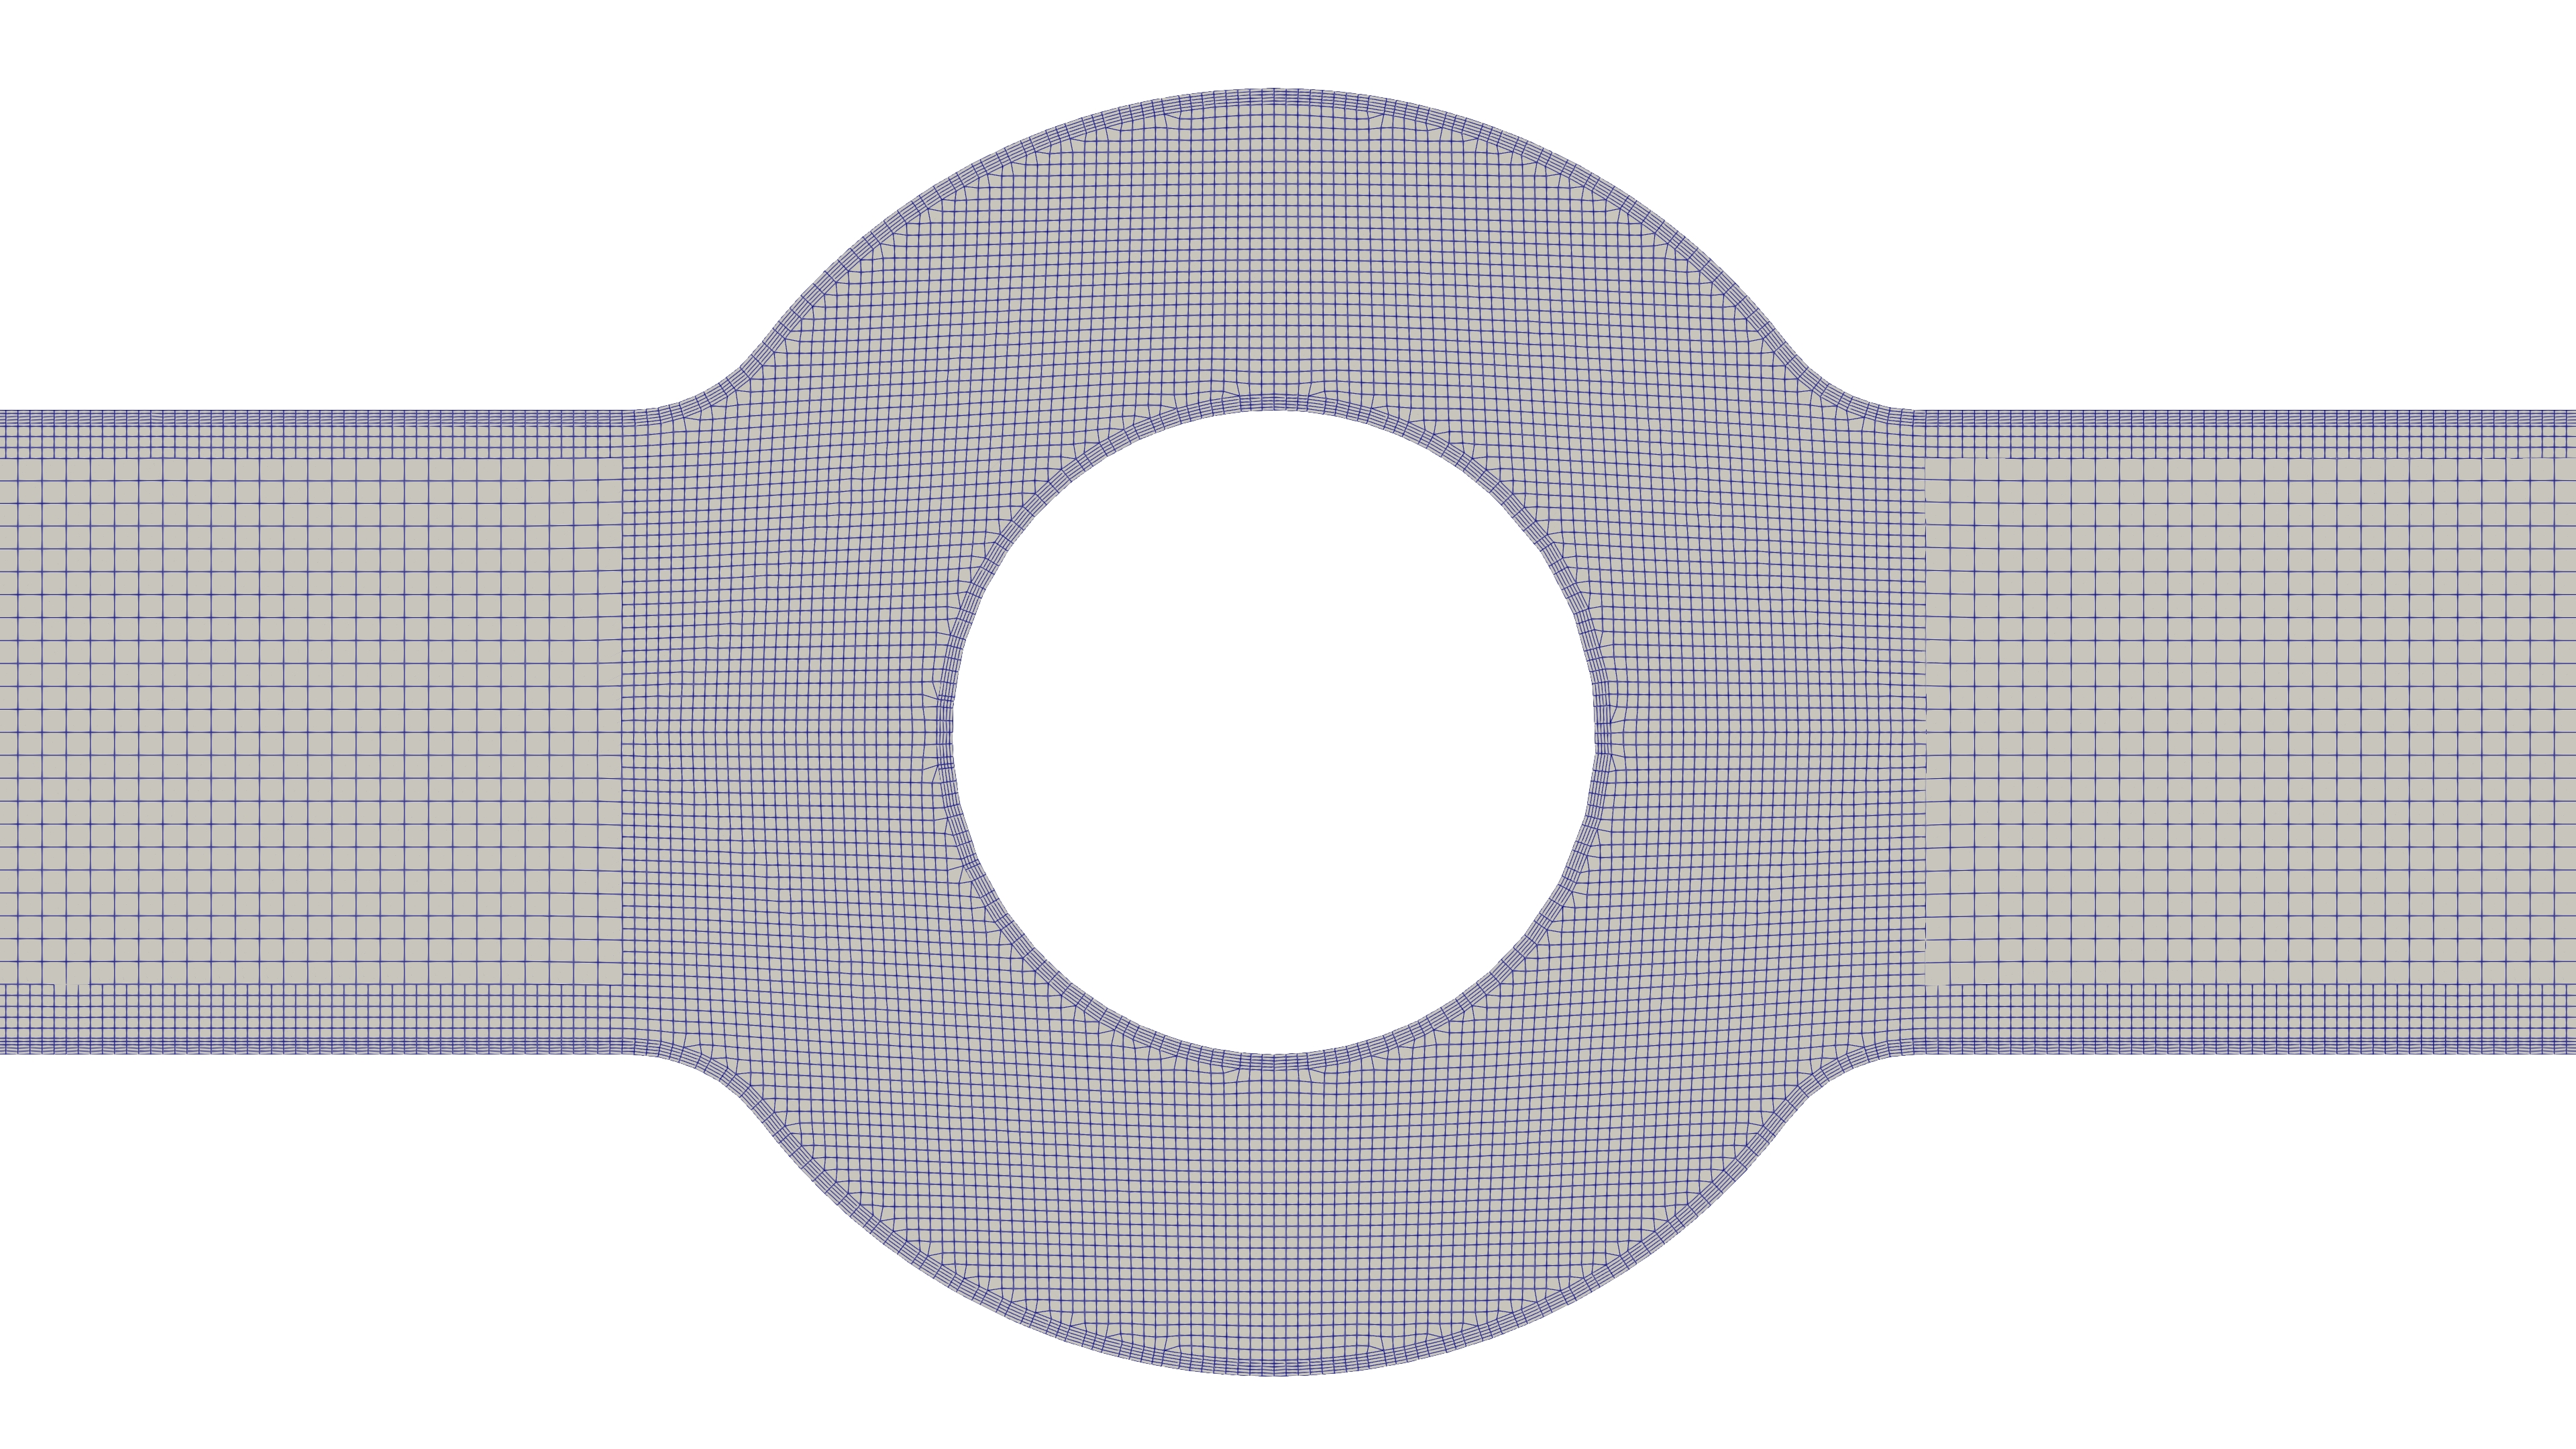
\includegraphics[width = 0.7\linewidth]{mesh}
         \caption{Расчетная сетка}
         \label{fig:mesh}
     \end{figure}
     
     Остаточная нефтенасыщенность в поре определяется в области, где возрастает плотность расчетной сетки(рис~\ref{fig:mesh}).
   
    \section*{Результаты}
    
    \begin{figure}[H]
        \centering
        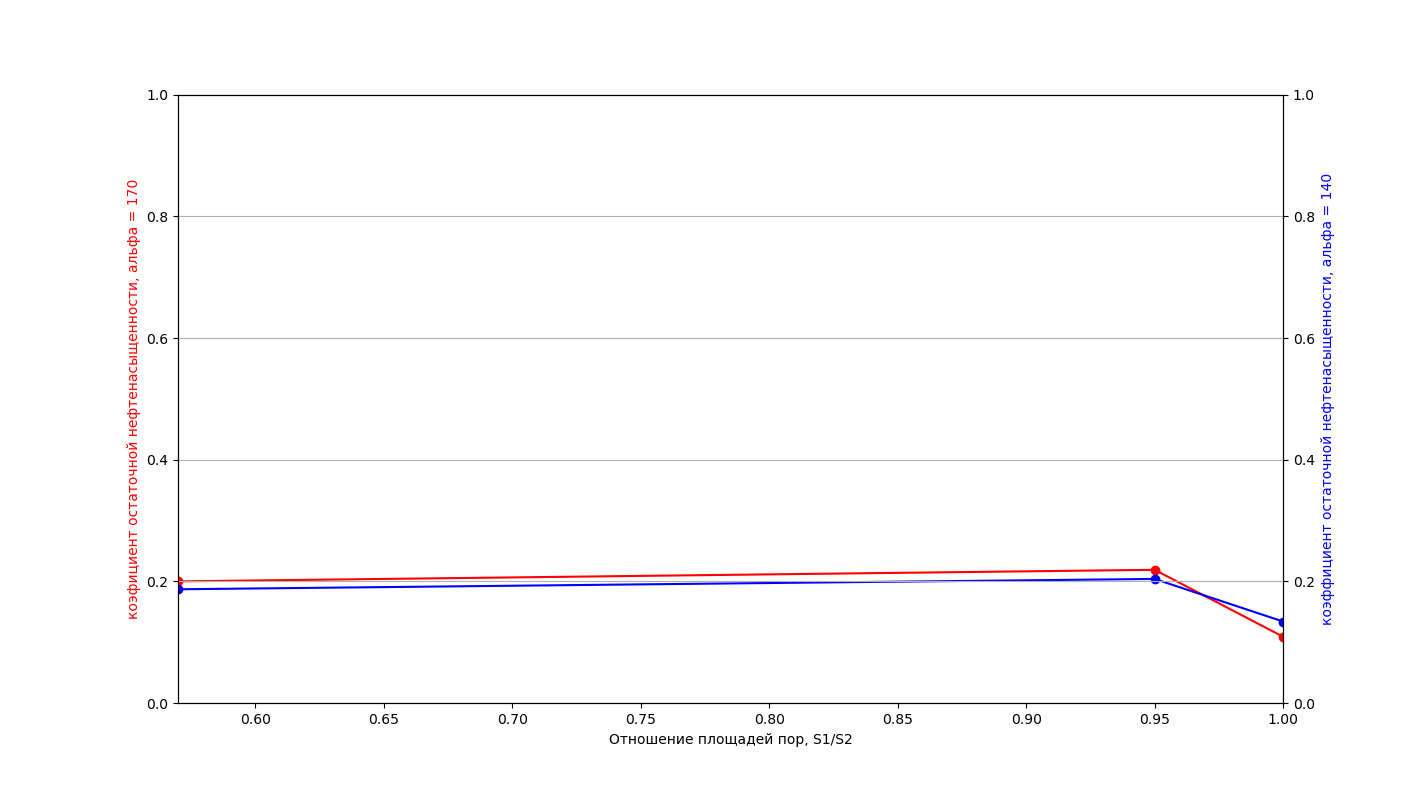
\includegraphics[width = 1\linewidth]{oil}
        \caption{Зависимость остаточной нефтенасыщенности от отношения площадей пор}
        \label{fig:oil}
    \end{figure}
    
    \begin{figure}[H]
        \centering
        
\includegraphics[width = 1\linewidth]{oilLeft}
        \caption{Остаточная нефтенасыщенность, S1/S2 = 0.57, $\alpha$ = 140}
        \label{fig:oilLeft}
    \end{figure}
    
    
    
    В дальнейшем исследовании планируется построение параметрической карты по которой, зная контактный угол и соотношение площадей пор, можно будет предсказывать остаточную нефтенасыщенность. Так же возможно и развитие параметрической модели с добавлением возможности построения геометрии через задание отношения площадей и характерные размеры одной поры для получения модели микроканала с предсказуемой нефтенасыщенностью. 
    
    
    
    
\end{document}